% !TEX program = xelatex
\PassOptionsToPackage{no-math}{fontspec}
\documentclass[a4paper,twocolumn,zihao=5,fontset=none,UTF8]{ctexart}
% Shared layout for the two Lab0 translations: Chinese two-column conference style.
\usepackage[a4paper,left=1.9cm,right=1.9cm,top=2.4cm,bottom=2.2cm,
  columnsep=0.7cm,headsep=0.5cm]{geometry}
\usepackage{amsmath,amssymb,bm}
\setmainfont{Times New Roman}
\setsansfont{Helvetica}
\setmonofont{Menlo}[Scale=0.85]
% macOS system CJK fonts; Kai/Fang come from TeX Live's Fandol set.
\setCJKmainfont{Songti SC}[BoldFont={Heiti SC},ItalicFont={FandolKai-Regular.otf}]
\setCJKsansfont{Heiti SC}
\setCJKmonofont{Heiti SC}
\setCJKfamilyfont{zhhei}{Heiti SC}
\setCJKfamilyfont{zhkai}{FandolKai-Regular.otf}
\setCJKfamilyfont{zhfs}{FandolFang-Regular.otf}
\providecommand{\heiti}{\CJKfamily{zhhei}}
\providecommand{\kaishu}{\CJKfamily{zhkai}}
\providecommand{\fangsong}{\CJKfamily{zhfs}}
\usepackage{newtxmath}
% fontspec's text fonts have no OT1 shapes; point math alphabets at newtx's Times.
\DeclareMathAlphabet{\mathrm}{OT1}{ntxtlf}{m}{n}
\DeclareMathAlphabet{\mathbf}{OT1}{ntxtlf}{b}{n}
\DeclareMathAlphabet{\mathtt}{OT1}{txtt}{m}{n}
\DeclareMathAlphabet{\mathsf}{OT1}{phv}{m}{n}
\SetSymbolFont{operators}{normal}{OT1}{ntxtlf}{m}{n}
\SetSymbolFont{operators}{bold}{OT1}{ntxtlf}{b}{n}
\usepackage{graphicx,booktabs,multirow,array}
\usepackage[font=small,labelsep=quad,skip=4pt]{caption}
\usepackage{enumitem}
\usepackage{fancyvrb}
\usepackage{fancyhdr}
\usepackage{xurl}
\usepackage[hidelinks]{hyperref}
\graphicspath{{figures/}}
\urlstyle{same}

\ctexset{
  section={format=\heiti\zihao{-4}\raggedright,beforeskip=1.2ex plus .3ex,
    afterskip=.8ex plus .2ex,aftername=\quad},
  subsection={format=\heiti\zihao{5}\raggedright,beforeskip=.9ex plus .2ex,
    afterskip=.5ex plus .1ex,aftername=\quad},
}
\setlist{nosep,leftmargin=2em}
\setlength{\parskip}{0pt}
\linespread{1.18}
\setlength{\abovedisplayskip}{5pt plus 2pt minus 2pt}
\setlength{\belowdisplayskip}{5pt plus 2pt minus 2pt}
\setlength{\textfloatsep}{10pt plus 2pt minus 3pt}
\setlength{\dbltextfloatsep}{10pt plus 2pt minus 3pt}
\emergencystretch=1em

% Bold run-in heading used by both papers ("Photogrammetric calibration." etc.).
\newcommand{\runin}[1]{\textbf{\heiti #1}\quad}
% Translator's note in a footnote.
\newcommand{\yizhe}[1]{\footnote{\kaishu 译者注：#1}}

\pagestyle{fancy}
\fancyhf{}
\renewcommand{\headrulewidth}{0.4pt}
\fancyfoot[C]{\small\thepage}


\fancyhead[L]{\small 机器人学集成小组项目 1 \quad Lab0-1 论文翻译}
\fancyhead[R]{\small 张正友：基于未知方位平面观测的灵活相机标定方法}

\newcommand{\A}{\mathbf{A}}
\newcommand{\B}{\mathbf{B}}
\newcommand{\Hm}{\mathbf{H}}
\newcommand{\R}{\mathbf{R}}
\newcommand{\h}{\mathbf{h}}
\newcommand{\rr}{\mathbf{r}}
\newcommand{\tv}{\mathbf{t}}
\newcommand{\bv}{\mathbf{b}}
\newcommand{\vvec}{\mathbf{v}}
\newcommand{\m}{\mathbf{m}}
\newcommand{\tm}{\widetilde{\mathbf{m}}}
\newcommand{\M}{\mathtt{M}}
\newcommand{\tM}{\widetilde{\mathtt{M}}}

\begin{document}

\twocolumn[{%
\begin{center}
  {\heiti\zihao{2} 基于未知方位平面观测的灵活相机标定方法\par}
  \vspace{0.5em}
  {\zihao{-4} Flexible Camera Calibration By Viewing a Plane From Unknown Orientations\par}
  \vspace{0.8em}
  {\fangsong\zihao{4} 张正友\,(Zhengyou Zhang)\par}
  \vspace{0.3em}
  {\zihao{-5} 微软研究院，One Microsoft Way, Redmond, WA 98052-6399, USA\quad
   zhang@microsoft.com\quad http://research.microsoft.com/\textasciitilde zhang\par}
\end{center}
\vspace{0.4em}
{\zihao{-5}\linespread{1.25}\selectfont
\noindent{\heiti 摘\quad 要：}本文提出一种能够方便地标定相机的灵活新技术。该技术只要求相机观测一个在少数几个（至少两个）不同方位下呈现的平面模板。相机和平面模板均可自由移动，且无须知道其运动。方法对镜头径向畸变进行了建模。所提出的流程先求取闭式解，再基于极大似然准则进行非线性精化。我们用计算机仿真和真实数据对该技术进行了测试，取得了非常好的结果。与使用两个或三个相互正交的平面等昂贵设备的经典技术相比，本文技术易于使用且灵活，推动三维计算机视觉从实验室环境向真实世界应用迈进了一步。相应的软件可从作者主页获取。

\vspace{0.3em}
\noindent{\heiti 关键词：}相机标定；内参数；镜头畸变；基于平面的灵活标定；运动分析；模型获取
\par}
\vspace{1.2em}
}]

{\renewcommand{\thefootnote}{}\footnotetext{\kaishu 原文：Z.~Zhang. Flexible Camera Calibration By Viewing a Plane From Unknown Orientations. Proc.\ 7th IEEE International Conference on Computer Vision (ICCV), 1999. 译者：许轩烨（学号 24020036071 / H00490299）。文中公式编号、图表编号与参考文献编号均与原文一致；译者补充的说明以“译者注”标出。}}

\section{研究动机}

相机标定是三维计算机视觉中从二维图像提取度量信息的必要步骤。围绕这一问题已有大量工作，最早始于摄影测量领域（例如文献[2, 4]），近年来则集中在计算机视觉领域（例如文献[9, 8, 20, 7, 23, 21, 15, 6, 19]）。这些技术大致可以分为两类：

\runin{摄影测量标定。}通过观测一个三维几何形状已知且精度很高的标定物来完成标定，标定过程可以非常高效[5]。标定物通常由两个或三个相互正交的平面组成；有时也使用一个做精确已知平移的平面[20]。这类方法需要昂贵的标定装置和精细的布置。

\runin{自标定。}这类技术不使用任何标定物。仅在静态场景中移动相机，场景的刚性一般就能只凭图像信息，从一次相机位移中得到关于相机内部参数的两个约束[15]。因此，若用内部参数固定的同一台相机拍摄图像，三幅图像之间的对应关系便足以同时恢复内部参数和外部参数，从而在相差一个相似变换的意义下重建三维结构[14, 12]。这种方法虽然非常灵活，但尚不成熟[1]。由于需要估计的参数很多，并不总能得到可靠的结果。

\runin{其他技术。}此外还有利用正交方向消失点的方法[3, 13]，以及基于纯旋转的标定方法[10, 18]。

我们目前的研究集中在桌面视觉系统（desktop vision system，DVS）上，因为 DVS 有着广阔的应用潜力。相机正变得廉价且无处不在。DVS 面向的是并非计算机视觉专家的普通大众。典型的计算机用户只是偶尔执行视觉任务，因而不愿为昂贵的设备投入资金。因此，灵活性、鲁棒性和低成本十分重要。本文所述的相机标定技术正是基于这些考虑而开发的。

本文提出的技术只要求相机观测一个在少数几个（至少两个）不同方位下呈现的平面模板。模板可以用激光打印机打印，并贴附在一个“合理”的平面表面上（例如硬质书籍封面）。相机或平面模板都可以用手移动，且无须知道其运动。由于我们使用的是二维度量信息，而不是三维信息或纯隐式信息，所提方法介于摄影测量标定与自标定之间。我们用计算机仿真和真实数据对该技术进行了测试，取得了非常好的结果。与经典技术相比，本文方法灵活得多；与自标定相比，它获得了相当程度的鲁棒性。我们相信，这一新技术推动三维计算机视觉从实验室环境向真实世界迈进了一步。

需要指出，Bill Triggs[19]最近提出了一种利用平面场景的至少 5 个视图进行自标定的技术。该技术比我们的更灵活，但难以初始化。Liebowitz 和 Zisserman[13]描述了一种对平面透视图像进行度量校正的技术，它利用一个已知角度、两个相等但未知的角度以及一个已知长度比等度量信息。他们还提到，只要得到这种经过度量校正的平面，就可以标定相机内部参数，但并未给出算法或实验结果。

本文结构如下：第 2 节描述观测单个平面所得到的基本约束；第 3 节描述标定流程，先求闭式解，再进行非线性优化，同时对镜头径向畸变建模；第 4 节研究使所提标定技术失效的配置，这些情况在实际中很容易避免；第 5 节给出实验结果，用计算机仿真和真实数据验证所提技术。附录给出若干细节，包括估计模型平面与其图像之间单应矩阵的技术。

\section{基本方程}

我们考察观测单个平面所得到的关于相机内参数的约束。首先说明本文所用的记号。

\subsection{记号}

二维点记为 $\m=[u,v]^T$，三维点记为 $\M=[X,Y,Z]^T$。用 $\widetilde{\mathbf{x}}$ 表示在末尾添加元素 1 后得到的增广向量：$\tm=[u,v,1]^T$，$\tM=[X,Y,Z,1]^T$。相机采用常用的针孔模型，三维点 $\M$ 与其图像投影 $\m$ 之间的关系为
\begin{equation}
  s\tm=\A\begin{bmatrix}\R & \tv\end{bmatrix}\tM
  \quad\text{其中}\quad
  \A=\begin{bmatrix}\alpha & c & u_0\\ 0 & \beta & v_0\\ 0 & 0 & 1\end{bmatrix}
\end{equation}
式中 $s$ 为任意尺度因子；$(\R,\tv)$ 称为外参数，是联系世界坐标系与相机坐标系的旋转和平移；$\A$ 称为相机内参数矩阵，其中 $(u_0,v_0)$ 为主点坐标，$\alpha$ 和 $\beta$ 分别为图像 $u$ 轴和 $v$ 轴上的尺度因子，$c$ 为描述两条图像坐标轴之间倾斜程度的参数。

我们用 $\A^{-T}$ 简记 $(\A^{-1})^T$ 或 $(\A^T)^{-1}$。

\subsection{模型平面与其图像之间的单应}

不失一般性，假设模型平面位于世界坐标系的 $Z=0$ 平面上。记旋转矩阵 $\R$ 的第 $i$ 列为 $\rr_i$。由式 (1) 可得
\begin{equation*}
  s\begin{bmatrix}u\\ v\\ 1\end{bmatrix}
  =\A\begin{bmatrix}\rr_1 & \rr_2 & \rr_3 & \tv\end{bmatrix}
   \begin{bmatrix}X\\ Y\\ 0\\ 1\end{bmatrix}
  =\A\begin{bmatrix}\rr_1 & \rr_2 & \tv\end{bmatrix}
   \begin{bmatrix}X\\ Y\\ 1\end{bmatrix}
\end{equation*}
在不致混淆的前提下，我们仍用 $\M$ 表示模型平面上的点，但由于 $Z$ 恒为 0，此时 $\M=[X,Y]^T$，相应地 $\tM=[X,Y,1]^T$。于是，模型点 $\M$ 与其图像点 $\m$ 之间由一个单应矩阵 $\Hm$ 相联系：
\begin{equation}
  s\tm=\Hm\tM\quad\text{其中}\quad \Hm=\A\begin{bmatrix}\rr_1 & \rr_2 & \tv\end{bmatrix}.
\end{equation}
显然，$3\times3$ 矩阵 $\Hm$ 只在相差一个尺度因子的意义下确定。

\subsection{内参数约束}

给定模型平面的一幅图像，就可以估计出一个单应矩阵（见附录 A）。将其记为 $\Hm=\begin{bmatrix}\h_1 & \h_2 & \h_3\end{bmatrix}$。由式 (2) 可得
\begin{equation*}
  \begin{bmatrix}\h_1 & \h_2 & \h_3\end{bmatrix}
  =\lambda\A\begin{bmatrix}\rr_1 & \rr_2 & \tv\end{bmatrix},
\end{equation*}
其中 $\lambda$ 为任意标量。利用 $\rr_1$ 与 $\rr_2$ 为单位正交向量这一性质，有
\begin{align}
  \h_1^T\A^{-T}\A^{-1}\h_2 &= 0\\
  \h_1^T\A^{-T}\A^{-1}\h_1 &= \h_2^T\A^{-T}\A^{-1}\h_2 .
\end{align}
这就是由一个单应矩阵得到的关于内参数的两个基本约束。由于单应矩阵有 8 个自由度，而外参数有 6 个（旋转 3 个、平移 3 个），因此只能得到关于内参数的 2 个约束。

\section{相机标定的求解}

本节详细说明如何有效地求解相机标定问题。我们先给出解析解，再给出基于极大似然准则的非线性优化技术，最后考虑镜头畸变，并同时给出其解析解和非线性解。

\subsection{闭式解}

令
\begin{equation}
\begin{aligned}
  \B&=\A^{-T}\A^{-1}\equiv
  \begin{bmatrix}B_{11} & B_{12} & B_{13}\\ B_{12} & B_{22} & B_{23}\\ B_{13} & B_{23} & B_{33}\end{bmatrix}\\
  &={\scriptstyle\begin{bmatrix}
    \frac{1}{\alpha^2} & -\frac{c}{\alpha^2\beta} & \frac{cv_0-u_0\beta}{\alpha^2\beta}\\[4pt]
    -\frac{c}{\alpha^2\beta} & \frac{c^2}{\alpha^2\beta^2}+\frac{1}{\beta^2} &
      -\frac{c(cv_0-u_0\beta)}{\alpha^2\beta^2}-\frac{v_0}{\beta^2}\\[4pt]
    \frac{cv_0-u_0\beta}{\alpha^2\beta} & -\frac{c(cv_0-u_0\beta)}{\alpha^2\beta^2}-\frac{v_0}{\beta^2} &
      \frac{(cv_0-u_0\beta)^2}{\alpha^2\beta^2}+\frac{v_0^2}{\beta^2}+1
  \end{bmatrix}}.
\end{aligned}
\end{equation}
注意 $\B$ 是对称矩阵，可由一个六维向量定义：
\begin{equation}
  \bv=[B_{11},B_{12},B_{22},B_{13},B_{23},B_{33}]^T .
\end{equation}
（它实际上描述的是绝对二次曲线的像。）

记 $\Hm$ 的第 $i$ 个列向量为 $\h_i=[h_{i1},h_{i2},h_{i3}]^T$，则有
\begin{equation}
  \h_i^T\B\h_j=\vvec_{ij}^T\bv
\end{equation}
其中
\begin{equation*}
\begin{aligned}
  \vvec_{ij}=[&h_{i1}h_{j1},\ h_{i1}h_{j2}+h_{i2}h_{j1},\ h_{i2}h_{j2},\\
  &h_{i3}h_{j1}+h_{i1}h_{j3},\ h_{i3}h_{j2}+h_{i2}h_{j3},\ h_{i3}h_{j3}]^T .
\end{aligned}
\end{equation*}
因此，由给定单应矩阵得到的两个基本约束 (3) 和 (4) 可以改写为关于 $\bv$ 的 2 个齐次方程：
\begin{equation}
  \begin{bmatrix}\vvec_{12}^T\\ (\vvec_{11}-\vvec_{22})^T\end{bmatrix}\bv=\mathbf{0}.
\end{equation}

若观测到模型平面的 $n$ 幅图像，将 $n$ 个形如 (8) 的方程堆叠起来，得到
\begin{equation}
  \mathbf{V}\bv=\mathbf{0},
\end{equation}
其中 $\mathbf{V}$ 为 $2n\times6$ 矩阵。若 $n\ge3$，一般可以得到在相差一个尺度因子意义下唯一的解 $\bv$。若 $n=2$，可以施加无倾斜约束 $c=0$，即 $[0,1,0,0,0,0]\bv=0$，并将其作为附加方程加入式 (9)。众所周知，式 (9) 的解是 $\mathbf{V}^T\mathbf{V}$ 最小特征值所对应的特征向量（等价地，是 $\mathbf{V}$ 最小奇异值所对应的右奇异向量）。

估计出 $\bv$ 后，即可计算相机内参数矩阵 $\A$，详见附录 B。

$\A$ 已知后，每幅图像的外参数便很容易计算。由式 (2) 得
\begin{equation*}
  \rr_1=\lambda\A^{-1}\h_1,\ \rr_2=\lambda\A^{-1}\h_2,\ \rr_3=\rr_1\times\rr_2,\ \tv=\lambda\A^{-1}\h_3
\end{equation*}
其中 $\lambda=1/\|\A^{-1}\h_1\|=1/\|\A^{-1}\h_2\|$。当然，由于数据中存在噪声，这样计算出的矩阵 $\R=[\rr_1,\rr_2,\rr_3]$ 一般并不满足旋转矩阵的性质。附录 C 描述了一种由一般 $3\times3$ 矩阵估计最佳旋转矩阵的方法。

\subsection{极大似然估计}

上述解是通过最小化一个没有物理意义的代数距离得到的。我们可以通过极大似然推断对其进行精化。

给定模型平面的 $n$ 幅图像，模型平面上有 $m$ 个点。假设图像点受到独立同分布噪声的污染，则极大似然估计可以通过最小化如下泛函得到：
\begin{equation}
  \sum_{i=1}^{n}\sum_{j=1}^{m}\bigl\|\m_{ij}-\hat{\m}(\A,\R_i,\tv_i,\M_j)\bigr\|^2,
\end{equation}
其中 $\hat{\m}(\A,\R_i,\tv_i,\M_j)$ 是点 $\M_j$ 按照式 (2) 在第 $i$ 幅图像中的投影。旋转 $\R$ 用一个三参数向量 $\rr$ 参数化，$\rr$ 平行于旋转轴，其模等于旋转角。$\R$ 与 $\rr$ 之间由 Rodrigues 公式相联系[5]。最小化式 (10) 是一个非线性最小化问题，我们用 \texttt{Minpack}[16] 中实现的 Levenberg-Marquardt 算法求解。该算法需要 $\A$ 和 $\{\R_i,\tv_i\,|\,i=1..n\}$ 的初始估计，这可以用上一小节所述的技术得到。

\subsection{径向畸变的处理}

到目前为止，我们尚未考虑相机的镜头畸变。然而，桌面相机通常存在明显的镜头畸变，尤其是径向畸变。本节只考虑径向畸变的前两项，更精细的模型请读者参阅文献[17, 2, 4, 23]。根据文献[2, 20, 22]的报道，畸变函数很可能完全由径向分量主导，尤其由第一项主导。研究还发现，任何更精细的建模不仅无益（与传感器量化误差相比可以忽略），反而会引起数值不稳定[20, 22]。

设 $(u,v)$ 为理想的（不可观测的、无畸变的）像素图像坐标，$(\breve u,\breve v)$ 为对应的实际观测图像坐标。类似地，$(x,y)$ 和 $(\breve x,\breve y)$ 分别为理想的（无畸变的）和实际的（有畸变的）归一化图像坐标。我们有[2, 22]
\begin{equation*}
\begin{aligned}
  \breve x&=x+x[k_1(x^2+y^2)+k_2(x^2+y^2)^2]\\
  \breve y&=y+y[k_1(x^2+y^2)+k_2(x^2+y^2)^2],
\end{aligned}
\end{equation*}
其中 $k_1$ 和 $k_2$ 为径向畸变系数。径向畸变的中心与主点相同。由 $\breve u=u_0+\alpha\breve x+c\breve y$ 和 $\breve v=v_0+\beta\breve y$ 可得
\begin{align}
  \breve u&=u+(u-u_0)[k_1(x^2+y^2)+k_2(x^2+y^2)^2]\\
  \breve v&=v+(v-v_0)[k_1(x^2+y^2)+k_2(x^2+y^2)^2].
\end{align}

\runin{交替估计径向畸变。}由于径向畸变预计较小，可以期望在简单忽略畸变的情况下，用 3.2 节所述的技术也能较好地估计其余 5 个内参数。因此，一种策略是在估计出其余参数之后再估计 $k_1$ 和 $k_2$。于是，由式 (11) 和 (12)，每幅图像中的每个点都给出两个方程：
\begin{equation*}
  \setlength{\arraycolsep}{1.5pt}
  \begin{bmatrix}(u-u_0)(x^2+y^2) & (u-u_0)(x^2+y^2)^2\\ (v-v_0)(x^2+y^2) & (v-v_0)(x^2+y^2)^2\end{bmatrix}
  \begin{bmatrix}k_1\\ k_2\end{bmatrix}
  =\begin{bmatrix}\breve u-u\\ \breve v-v\end{bmatrix}.
\end{equation*}
给定 $n$ 幅图像中的 $m$ 个点，把所有方程堆叠起来，共得到 $2mn$ 个方程，写成矩阵形式为 $\mathbf{D}\mathbf{k}=\mathbf{d}$，其中 $\mathbf{k}=[k_1,k_2]^T$。其线性最小二乘解为
\begin{equation}
  \mathbf{k}=(\mathbf{D}^T\mathbf{D})^{-1}\mathbf{D}^T\mathbf{d}.
\end{equation}
估计出 $k_1$ 和 $k_2$ 后，可以把式 (10) 中的 $\hat{\m}(\A,\R_i,\tv_i,\M_j)$ 替换为式 (11) 和 (12)，求解式 (10) 以精化其余参数的估计。交替执行这两个步骤，直至收敛。

\runin{完整的极大似然估计。}实验中我们发现，上述交替技术收敛较慢。因此，对式 (10) 的一个自然扩展是通过最小化如下泛函来估计全部参数：
\begin{equation}
  \sum_{i=1}^{n}\sum_{j=1}^{m}\bigl\|\m_{ij}-\breve{\m}(\A,k_1,k_2,\R_i,\tv_i,\M_j)\bigr\|^2,
\end{equation}
其中 $\breve{\m}(\A,k_1,k_2,\R_i,\tv_i,\M_j)$ 是点 $\M_j$ 先按式 (2) 投影到第 $i$ 幅图像、再按式 (11) 和 (12) 施加畸变后得到的投影。这是一个非线性最小化问题，我们用 \texttt{Minpack}[16] 中实现的 Levenberg-Marquardt 算法求解。与 3.2 节相同，旋转仍用三维向量 $\rr$ 参数化。$\A$ 和 $\{\R_i,\tv_i\,|\,i=1..n\}$ 的初始估计可以用 3.1 节或 3.2 节所述的技术获得；$k_1$ 和 $k_2$ 的初始估计可以用上一段所述的技术获得，也可以简单地设为 0。

\subsection{小结}

推荐的标定流程如下：
\begin{enumerate}
  \item 打印一个模板，并将其贴附在平面表面上；
  \item 通过移动平面或相机，在不同方位下拍摄模型平面的若干幅图像；
  \item 检测图像中的特征点；
  \item 用 3.1 节所述的闭式解估计 5 个内参数和全部外参数；
  \item 求解线性最小二乘问题 (13)，估计径向畸变系数；
  \item 最小化式 (14)，精化全部参数。
\end{enumerate}

\section{退化配置}

本节研究这样一类配置：在这些配置下，增加图像不能为相机内参数提供更多约束。由于式 (3) 和 (4) 是由旋转矩阵的性质推导出来的，若 $\R_2$ 与 $\R_1$ 不独立，则图像 2 不能提供额外的约束。特别地，若平面只做纯平移，则 $\R_2=\R_1$，图像 2 对相机标定没有帮助。下面考虑一种更复杂的配置。

\noindent{\heiti 命题 1}\quad{\kaishu 若模型平面在第二个位置时与其第一个位置平行，则第二个单应矩阵不能提供额外的约束。}

\begin{figure}[t]
  \centering
  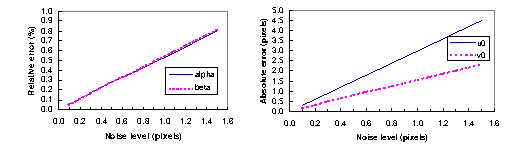
\includegraphics[width=\linewidth]{zhang_fig1}
  \caption{误差随图像点噪声水平的变化}
\end{figure}

由于篇幅所限，此处略去证明，证明可见我们的技术报告[24]。在实际中很容易避免这种退化配置：只需在每次拍摄时改变模型平面的方位即可。

\section{实验结果}

我们用计算机仿真数据和真实数据对所提算法进行了测试。闭式解只需对一个规模很小的 $2n\times6$ 矩阵做奇异值分解，其中 $n$ 为图像数目。Levenberg-Marquardt 算法中的非线性精化需要 3 到 5 次迭代即可收敛。

\subsection{计算机仿真}

仿真相机的参数如下：$\alpha=1250$，$\beta=900$，$c=1.09083$（相当于 $89.95^\circ$），$u_0=255$，$v_0=255$。图像分辨率为 $512\times512$。模型平面是一个包含 $10\times14=140$ 个角点的棋盘格模板（因此 $v$ 方向上的数据通常多于 $u$ 方向）。模板尺寸为 $18\,\text{cm}\times25\,\text{cm}$。平面的方位用三维向量 $\rr$ 表示，$\rr$ 平行于旋转轴，其模等于旋转角；平面的位置用三维向量 $\tv$ 表示（单位为厘米）。

\runin{噪声水平对性能的影响。}本实验使用三个平面，其参数为 $\rr_1=[20^\circ,0,0]^T$，$\tv_1=[-9,-12.5,500]^T$，$\rr_2=[0,20^\circ,0]^T$，$\tv_2=[-9,-12.5,510]^T$，$\rr_3=\frac{1}{\sqrt5}[-30^\circ,-30^\circ,-15^\circ]^T$，$\tv_3=[-10.5,-12.5,525]^T$。在投影得到的图像点上加入均值为 0、标准差为 $\sigma$ 的高斯噪声，然后将估计出的相机参数与真值比较。对 $\alpha$ 和 $\beta$ 度量相对误差，对 $u_0$ 和 $v_0$ 度量绝对误差。噪声水平从 0.1 像素变化到 1.5 像素。对每个噪声水平进行 100 次独立试验，所示结果为其平均值。从图 1 可以看出，误差随噪声水平线性增大（$c$ 的误差未画出，但具有相同的性质）。当 $\sigma=0.5$ 时（这已大于实际标定中的通常噪声），$\alpha$ 和 $\beta$ 的误差小于 0.3\%，$u_0$ 和 $v_0$ 的误差约为 1 像素。$u_0$ 的误差大于 $v_0$ 的误差，其主要原因正如前文所述，$u$ 方向上的数据少于 $v$ 方向。

\begin{figure}[t]
  \centering
  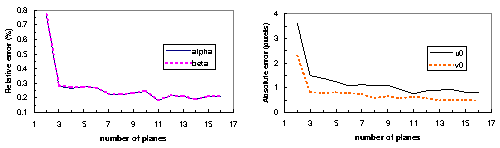
\includegraphics[width=\linewidth]{zhang_fig2}
  \caption{误差随模型平面图像数目的变化}
  \vspace{6pt}
  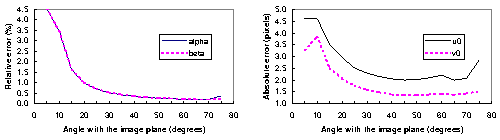
\includegraphics[width=\linewidth]{zhang_fig3}
  \caption{误差随模型平面相对像平面夹角的变化}
\end{figure}

\runin{平面数目对性能的影响。}本实验研究性能与平面数目（更确切地说，是模型平面图像的数目）的关系。前三幅图像中模型平面的方位和位置与上一小节相同。从第四幅图像开始，我们先在均匀球面上随机选取一个旋转轴，再施加 $30^\circ$ 的旋转角。图像数目从 2 变化到 16。对每个数目进行 100 次试验，其中平面方位（前三个除外）相互独立，并加入独立的、均值为 0、标准差为 0.5 像素的噪声。平均结果如图 2 所示。使用的图像越多，误差越小；从 2 幅增加到 3 幅时，误差显著减小。

\runin{模型平面方位对性能的影响。}本实验考察模型平面相对于像平面的方位的影响。使用 3 幅图像，平面方位按如下方式选取：平面初始时与像平面平行；从均匀球面上随机选取一个旋转轴；然后使平面绕该轴旋转角度 $\theta$。在投影得到的图像点上加入均值为 0、标准差为 0.5 像素的高斯噪声。重复该过程 100 次并计算平均误差。角度 $\theta$ 从 $5^\circ$ 变化到 $75^\circ$，结果如图 3 所示。当 $\theta=5^\circ$ 时，由于各平面几乎相互平行（退化配置），40\% 的试验失败，所示结果已剔除这些试验。角度约为 $45^\circ$ 时性能似乎最好。需要注意，在实际中，角度增大时透视缩短效应会降低角点检测的精度，但本实验没有考虑这一点。

\subsection{真实数据}

所提技术目前已在我们的视觉组和图形组中得到日常使用。这里给出一个例子的结果。

待标定的相机是一台配备 6\,mm 镜头的现成 PULNiX CCD 相机，图像分辨率为 $640\times480$。模型平面包含由 $8\times8$ 个正方形组成的模板，因此共有 256 个角点。模板尺寸为 $17\,\text{cm}\times17\,\text{cm}$。我们在不同方位下拍摄了该平面的 5 幅图像，如图 4 所示。可以看到图像中存在明显的镜头畸变。角点的检测方法是：对每个正方形的各边拟合直线，再求这些直线的交点。

\begin{figure*}[t]
  \centering
  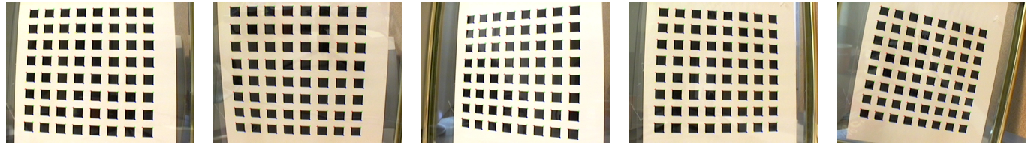
\includegraphics[width=\textwidth]{zhang_fig4}
  \caption{模型平面的 5 幅图像及提取出的角点（角点以十字标出，但十字太小而难以看清）}
\end{figure*}

\begin{table*}[t]
  \centering
  \caption{使用 2 至 5 幅真实图像的标定结果}
  \small
  \setlength{\tabcolsep}{4.2pt}
  \begin{tabular}{c|rrr|rrr|rrr|rrr}
    \toprule
    图像数 & \multicolumn{3}{c|}{2 幅图像} & \multicolumn{3}{c|}{3 幅图像} & \multicolumn{3}{c|}{4 幅图像} & \multicolumn{3}{c}{5 幅图像}\\
     & 初值 & 终值 & $\sigma$ & 初值 & 终值 & $\sigma$ & 初值 & 终值 & $\sigma$ & 初值 & 终值 & $\sigma$\\
    \midrule
    $\alpha$ & 825.59 & 830.47 & 4.74 & 917.65 & 830.80 & 2.06 & 876.62 & 831.81 & 1.56 & 877.16 & 832.50 & 1.41\\
    $\beta$ & 825.26 & 830.24 & 4.85 & 920.53 & 830.69 & 2.10 & 876.22 & 831.82 & 1.55 & 876.80 & 832.53 & 1.38\\
    $c$ & 0 & 0 & 0 & 2.2956 & 0.1676 & 0.109 & 0.0658 & 0.2867 & 0.095 & 0.1752 & 0.2045 & 0.078\\
    $u_0$ & 295.79 & 307.03 & 1.37 & 277.09 & 305.77 & 1.45 & 301.31 & 304.53 & 0.86 & 301.04 & 303.96 & 0.71\\
    $v_0$ & 217.69 & 206.55 & 0.93 & 223.36 & 206.42 & 1.00 & 220.06 & 206.79 & 0.78 & 220.41 & 206.56 & 0.66\\
    $k_1$ & 0.161 & $-0.227$ & 0.006 & 0.128 & $-0.229$ & 0.006 & 0.145 & $-0.229$ & 0.005 & 0.136 & $-0.228$ & 0.003\\
    $k_2$ & $-1.955$ & 0.194 & 0.032 & $-1.986$ & 0.196 & 0.034 & $-2.089$ & 0.195 & 0.028 & $-2.042$ & 0.190 & 0.025\\
    \midrule
    RMS & 0.761 & \multicolumn{2}{c|}{0.295} & 0.987 & \multicolumn{2}{c|}{0.393} & 0.927 & \multicolumn{2}{c|}{0.361} & 0.881 & \multicolumn{2}{c}{0.335}\\
    \bottomrule
  \end{tabular}

  \vspace{10pt}
  \caption{在所有图像四元组上标定结果的变化}
  \begin{tabular}{c|rrrrr|rr}
    \toprule
    四元组 & (1234) & (1235) & (1245) & (1345) & (2345) & 均值 & 标准差\\
    \midrule
    $\alpha$ & 831.81 & 832.09 & 837.53 & 829.69 & 833.14 & 832.85 & 2.90\\
    $\beta$ & 831.82 & 832.10 & 837.53 & 829.91 & 833.11 & 832.90 & 2.84\\
    $c$ & 0.2867 & 0.1069 & 0.0611 & 0.1363 & 0.1096 & 0.1401 & 0.086\\
    $u_0$ & 304.53 & 304.32 & 304.57 & 303.95 & 303.53 & 304.18 & 0.44\\
    $v_0$ & 206.79 & 206.23 & 207.30 & 207.16 & 206.33 & 206.76 & 0.48\\
    $k_1$ & $-0.229$ & $-0.228$ & $-0.230$ & $-0.227$ & $-0.229$ & $-0.229$ & 0.001\\
    $k_2$ & 0.195 & 0.191 & 0.193 & 0.179 & 0.190 & 0.190 & 0.006\\
    \midrule
    RMS & 0.361 & 0.357 & 0.262 & 0.358 & 0.334 & 0.334 & 0.04\\
    \bottomrule
  \end{tabular}
\end{table*}

我们分别用前 2、3、4 幅以及全部 5 幅图像运行标定算法，结果如表 1 所示。对每种配置给出三列：第一列（初值，initial）为闭式解的估计值；第二列（终值，final）为极大似然估计（MLE）；第三列（$\sigma$）为估计的标准差，表示最终结果的不确定度。可以看出，闭式解是合理的，而且无论使用 2、3、4 还是 5 幅图像，最终估计都非常一致。我们还注意到，最终估计的不确定度随图像数目的增加而减小。表 1 最后一行 RMS 表示检测到的图像点与投影点之间距离的均方根，单位为像素。MLE 显著改善了这一指标。

细心的读者可能会注意到，$k_1$ 和 $k_2$ 在闭式解与 MLE 之间并不一致。原因在于：闭式解是在假设无畸变的情况下估计相机内参数的，因而预测的外围点比检测到的点更靠近图像中心。随后的畸变估计试图把外围点向外推开、增大尺度以减小距离，尽管这种畸变形状（$k_1$ 为正，称为枕形畸变）与真实畸变（$k_1$ 为负，称为桶形畸变）并不相符。非线性精化（MLE）最终恢复了正确的畸变形状。利用估计出的畸变参数，可以校正原始图像中的畸变。图 5 给出了前两幅经畸变校正的图像，请将其与图 4 中的前两幅图像对比。可以清楚地看到，原始图像中弯曲的模板被拉直了。

\begin{figure}[t]
  \centering
  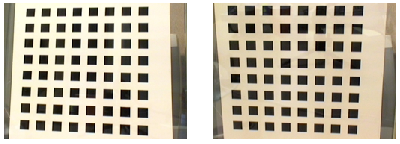
\includegraphics[width=0.92\linewidth]{zhang_fig5}
  \caption{校正径向畸变后的第一幅和第二幅图像}
\end{figure}

\runin{标定结果的变化。}表 1 给出了用 2 至 5 幅图像得到的标定结果，可以发现这些结果彼此非常一致。为了进一步考察所提算法的稳定性，我们把它应用于从现有 5 幅图像中任取 4 幅的所有组合，结果如表 2 所示。例如，第三列 (1235) 是用第 1、2、3、5 幅图像组成的四元组得到的结果。最后两列为五组结果的均值和样本标准差。所有参数的样本标准差都相当小，这表明所提算法相当稳定。倾斜参数 $c$ 的值与 0 没有显著差异，因为其变异系数 $0.086/0.1401=0.6$ 较大。事实上，$c=0.1401$、$\alpha=832.85$ 对应的两条图像坐标轴夹角为 89.99°，非常接近 90°。我们还对每个四元组计算了纵横比 $\alpha/\beta$，其均值为 0.99995，样本标准差为 0.00012，因此非常接近 1，即像素是正方形的。

\runin{在基于图像的建模中的应用。}我们用上述标定所用的同一台相机拍摄了一个茶叶罐的两幅图像（见图 6），图中主要可见其两个侧面。我们在每个侧面上手工选取了 8 对匹配点，并在这 16 对匹配点上运行我们早先开发的运动恢复结构（structure-from-motion）软件，建立了茶叶罐的部分模型。重建模型为 VRML 格式，图 7 给出了三个渲染视图。每个侧面上的重建点确实共面；我们计算了两个重建平面之间的夹角，为 $94.7^\circ$。虽然没有真值，但茶叶罐的两个侧面确实几乎相互正交。

\begin{figure}[t]
  \centering
  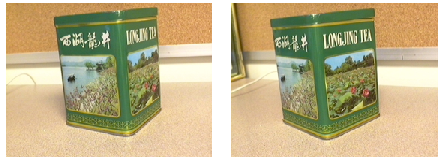
\includegraphics[width=0.95\linewidth]{zhang_fig6}
  \caption{茶叶罐的两幅图像}
  \vspace{6pt}
  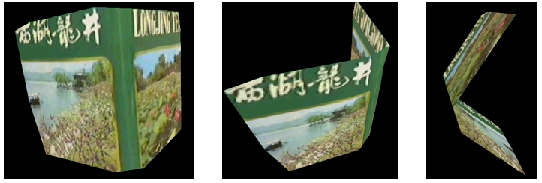
\includegraphics[width=0.95\linewidth]{zhang_fig7}
  \caption{重建茶叶罐的三个渲染视图}
\end{figure}

所有真实数据、结果以及软件均可从以下网页获取：\url{http://research.microsoft.com/~zhang/Calib/}

\section{结论}

本文提出了一种能够方便地标定相机的灵活新技术。该技术只要求相机从少数几个（至少两个）不同方位观测一个平面模板。相机或平面模板均可移动，且无须知道其运动。方法对镜头径向畸变进行了建模。所提出的流程由闭式解和随后基于极大似然准则的非线性精化组成。我们用计算机仿真和真实数据对该技术进行了测试，取得了非常好的结果。与使用两个或三个相互正交的平面等昂贵设备的经典技术相比，所提技术的灵活性大为提高。

\vspace{0.5em}
\noindent{\heiti 致谢}\quad 感谢 Brian Guenter 提供角点提取软件并进行了多次讨论，感谢 Bill Triggs 提出的深刻意见。感谢 Andrew Zisserman 使作者注意到他在 CVPR98 上发表的工作[13]，该工作使用了相同的约束，但形式不同。感谢 Bill Triggs 和 Gideon Stein 建议开展关于模型不精确性的实验，相关内容见技术报告[24]。Anandan 和 Charles Loop 检查了早期版本的英文。

\appendix
\ctexset{section/name={附录\,,},section/number=\Alph{section}}

\section{模型平面与其图像之间单应矩阵的估计}

估计模型平面与其图像之间单应矩阵的方法有很多，这里给出一种基于极大似然准则的技术。设 $\M_i$ 和 $\m_i$ 分别为模型点和图像点。理想情况下，它们应满足式 (2)；但实际上，由于提取的图像点含有噪声，它们并不严格满足该式。假设 $\m_i$ 受到均值为 $\mathbf{0}$、协方差矩阵为 $\Lambda_{\m_i}$ 的高斯噪声污染，则 $\Hm$ 的极大似然估计可以通过最小化如下泛函得到：
\begin{equation*}
  \sum_i(\m_i-\hat{\m}_i)^T\Lambda_{\m_i}^{-1}(\m_i-\hat{\m}_i),
\end{equation*}
\begin{equation*}
  \text{其中}\ \hat{\m}_i=\frac{1}{\bar{\h}_3^T\tM_i}
  \begin{bmatrix}\bar{\h}_1^T\tM_i\\ \bar{\h}_2^T\tM_i\end{bmatrix},
  \quad \bar{\h}_i\ \text{为}\ \Hm\ \text{的第}\ i\ \text{行}.
\end{equation*}

实际中，我们简单地假设对所有 $i$ 有 $\Lambda_{\m_i}=\sigma^2\mathbf{I}$。如果各点是用相同的过程独立提取的，这一假设是合理的。此时，上述问题变为一个非线性最小二乘问题，即 $\min_{\Hm}\sum_i\|\m_i-\hat{\m}_i\|^2$。该非线性最小化用 \texttt{Minpack}[16] 中实现的 Levenberg-Marquardt 算法求解，它需要一个初始估计，可按如下方法得到。

令 $\mathbf{x}=[\bar{\h}_1^T,\bar{\h}_2^T,\bar{\h}_3^T]^T$，则式 (2) 可以改写为
\begin{equation*}
  \begin{bmatrix}\tM^T & \mathbf{0}^T & -u\tM^T\\ \mathbf{0}^T & \tM^T & -v\tM^T\end{bmatrix}\mathbf{x}=\mathbf{0}.
\end{equation*}
给定 $n$ 个点时，有 $n$ 组上述方程，可以写成矩阵方程 $\mathbf{L}\mathbf{x}=\mathbf{0}$，其中 $\mathbf{L}$ 为 $2n\times9$ 矩阵。由于 $\mathbf{x}$ 只在相差一个尺度因子的意义下确定，众所周知，其解为 $\mathbf{L}$ 最小奇异值所对应的右奇异向量（等价地，为 $\mathbf{L}^T\mathbf{L}$ 最小特征值所对应的特征向量）。

在 $\mathbf{L}$ 中，有些元素是常数 1，有些以像素为单位，有些以世界坐标为单位，还有些是两者的乘积，这使得 $\mathbf{L}$ 在数值上是病态的。在执行上述过程之前先做简单的数据归一化（例如文献[11]提出的方法），可以得到好得多的结果。

\section{由矩阵 B 提取内参数}

如 3.1 节所述，矩阵 $\B$ 是在相差一个尺度因子的意义下估计的，即 $\B=\lambda\A^{-T}\A$\yizhe{按式 (5) 的定义，此处应为 $\B=\lambda\A^{-T}\A^{-1}$。}，其中 $\lambda$ 为任意尺度。我们可以毫无困难地从矩阵 $\B$ 中唯一地提取出内参数：
\begin{equation*}
\begin{aligned}
  v_0&=(B_{12}B_{13}-B_{11}B_{23})/(B_{11}B_{22}-B_{12}^2)\\
  \lambda&=B_{33}-[B_{13}^2+v_0(B_{12}B_{13}-B_{11}B_{23})]/B_{11}\\
  \alpha&=\sqrt{\lambda/B_{11}}\\
  \beta&=\sqrt{\lambda B_{11}/(B_{11}B_{22}-B_{12}^2)}\\
  c&=-B_{12}\alpha^2\beta/\lambda\\
  u_0&=cv_0/\alpha-B_{13}\alpha^2/\lambda.\footnotemark
\end{aligned}
\end{equation*}
\footnotetext{\kaishu 译者注：由式 (5) 中 $B_{13}=(cv_0-u_0\beta)/(\alpha^2\beta)$ 可推得 $u_0=cv_0/\beta-B_{13}\alpha^2/\lambda$，即最后一式第一项的分母应为 $\beta$ 而非 $\alpha$。实际相机中 $\alpha\approx\beta$ 且 $c\approx0$，两者的数值差异通常很小。}

\section{用旋转矩阵近似 3×3 矩阵}

本节考虑的问题是：求一个最佳旋转矩阵 $\R$，用以近似给定的 $3\times3$ 矩阵 $\mathbf{Q}$。这里的“最佳”是指差 $\R-\mathbf{Q}$ 的 Frobenius 范数最小。解法可见我们的技术报告[24]。

\section*{参考文献}
\begingroup
\small
\renewcommand{\refname}{}
\begin{enumerate}[label={[\arabic*]},leftmargin=2.2em,itemsep=1pt]
\item S. Bougnoux. From projective to euclidean space under any practical situation, a criticism of self-calibration. In \emph{Proc.\ 6th International Conference on Computer Vision}, pages 790--796, Jan.\ 1998.
\item D. C. Brown. Close-range camera calibration. \emph{Photogrammetric Engineering}, 37(8):855--866, 1971.
\item B. Caprile and V. Torre. Using Vanishing Points for Camera Calibration. \emph{The International Journal of Computer Vision}, 4(2):127--140, Mar.\ 1990.
\item W. Faig. Calibration of close-range photogrammetry systems: Mathematical formulation. \emph{Photogrammetric Engineering and Remote Sensing}, 41(12):1479--1486, 1975.
\item O. Faugeras. \emph{Three-Dimensional Computer Vision: a Geometric Viewpoint}. MIT Press, 1993.
\item O. Faugeras, T. Luong, and S. Maybank. Camera self-calibration: theory and experiments. In \emph{Proc.\ 2nd ECCV}, pages 321--334, May 1992.
\item O. Faugeras and G. Toscani. The calibration problem for stereo. In \emph{Proc.\ IEEE Conference on Computer Vision and Pattern Recognition}, pages 15--20, Miami Beach, FL, June 1986.
\item S. Ganapathy. Decomposition of transformation matrices for robot vision. \emph{Pattern Recognition Letters}, 2:401--412, Dec.\ 1984.
\item D. Gennery. Stereo-camera calibration. In \emph{Proc.\ 10th Image Understanding Workshop}, pages 101--108, 1979.
\item R. Hartley. Self-calibration from multiple views with a rotating camera. In \emph{Proc.\ 3rd European Conference on Computer Vision}, pages 471--478, Stockholm, Sweden, May 1994.
\item R. Hartley. In defence of the 8-point algorithm. In \emph{Proc.\ 5th International Conference on Computer Vision}, pages 1064--1070, Boston, MA, June 1995.
\item R. I. Hartley. An algorithm for self calibration from several views. In \emph{Proc.\ IEEE Conference on Computer Vision and Pattern Recognition}, pages 908--912, Seattle, WA, June 1994.
\item D. Liebowitz and A. Zisserman. Metric rectification for perspective images of planes. In \emph{Proc.\ IEEE Conference on Computer Vision and Pattern Recognition}, pages 482--488, Santa Barbara, California, June 1998.
\item Q.-T. Luong and O. Faugeras. Self-calibration of a moving camera from point correspondences and fundamental matrices. \emph{The International Journal of Computer Vision}, 22(3):261--289, 1997.
\item S. J. Maybank and O. D. Faugeras. A theory of self-calibration of a moving camera. \emph{The International Journal of Computer Vision}, 8(2):123--152, Aug.\ 1992.
\item J. More. The levenberg-marquardt algorithm, implementation and theory. In G. A. Watson, editor, \emph{Numerical Analysis}, Lecture Notes in Mathematics 630. Springer-Verlag, 1977.
\item C. C. Slama, editor. \emph{Manual of Photogrammetry}. American Society of Photogrammetry, 4th ed., 1980.
\item G. Stein. Accurate internal camera calibration using rotation, with analysis of sources of error. In \emph{Proc.\ 5th International Conference on Computer Vision}, pages 230--236, Cambridge, Massachusetts, June 1995.
\item B. Triggs. Autocalibration from planar scenes. In \emph{Proc.\ 5th European Conference on Computer Vision}, pages 89--105, Freiburg, Germany, June 1998.
\item R. Y. Tsai. A versatile camera calibration technique for high-accuracy 3D machine vision metrology using off-the-shelf tv cameras and lenses. \emph{IEEE Journal of Robotics and Automation}, 3(4):323--344, Aug.\ 1987.
\item G. Wei and S. Ma. A complete two-plane camera calibration method and experimental comparisons. In \emph{Proc.\ Fourth International Conference on Computer Vision}, pages 439--446, Berlin, May 1993.
\item G. Wei and S. Ma. Implicit and explicit camera calibration: Theory and experiments. \emph{IEEE Transactions on Pattern Analysis and Machine Intelligence}, 16(5):469--480, 1994.
\item J. Weng, P. Cohen, and M. Herniou. Camera calibration with distortion models and accuracy evaluation. \emph{IEEE Transactions on Pattern Analysis and Machine Intelligence}, 14(10):965--980, Oct.\ 1992.
\item Z. Zhang. \emph{A Flexible New Technique for Camera Calibration}. Technical Report MSR-TR-98-71, Microsoft Research, December 1998. Available together with the software at \url{http://research.microsoft.com/~zhang/Calib/}
\end{enumerate}
\endgroup

\end{document}
